%!TEX root = ../Thesis.tex
\section{Das Team mit Namen und Bild}

\vfill

\begin{figure}[h]
	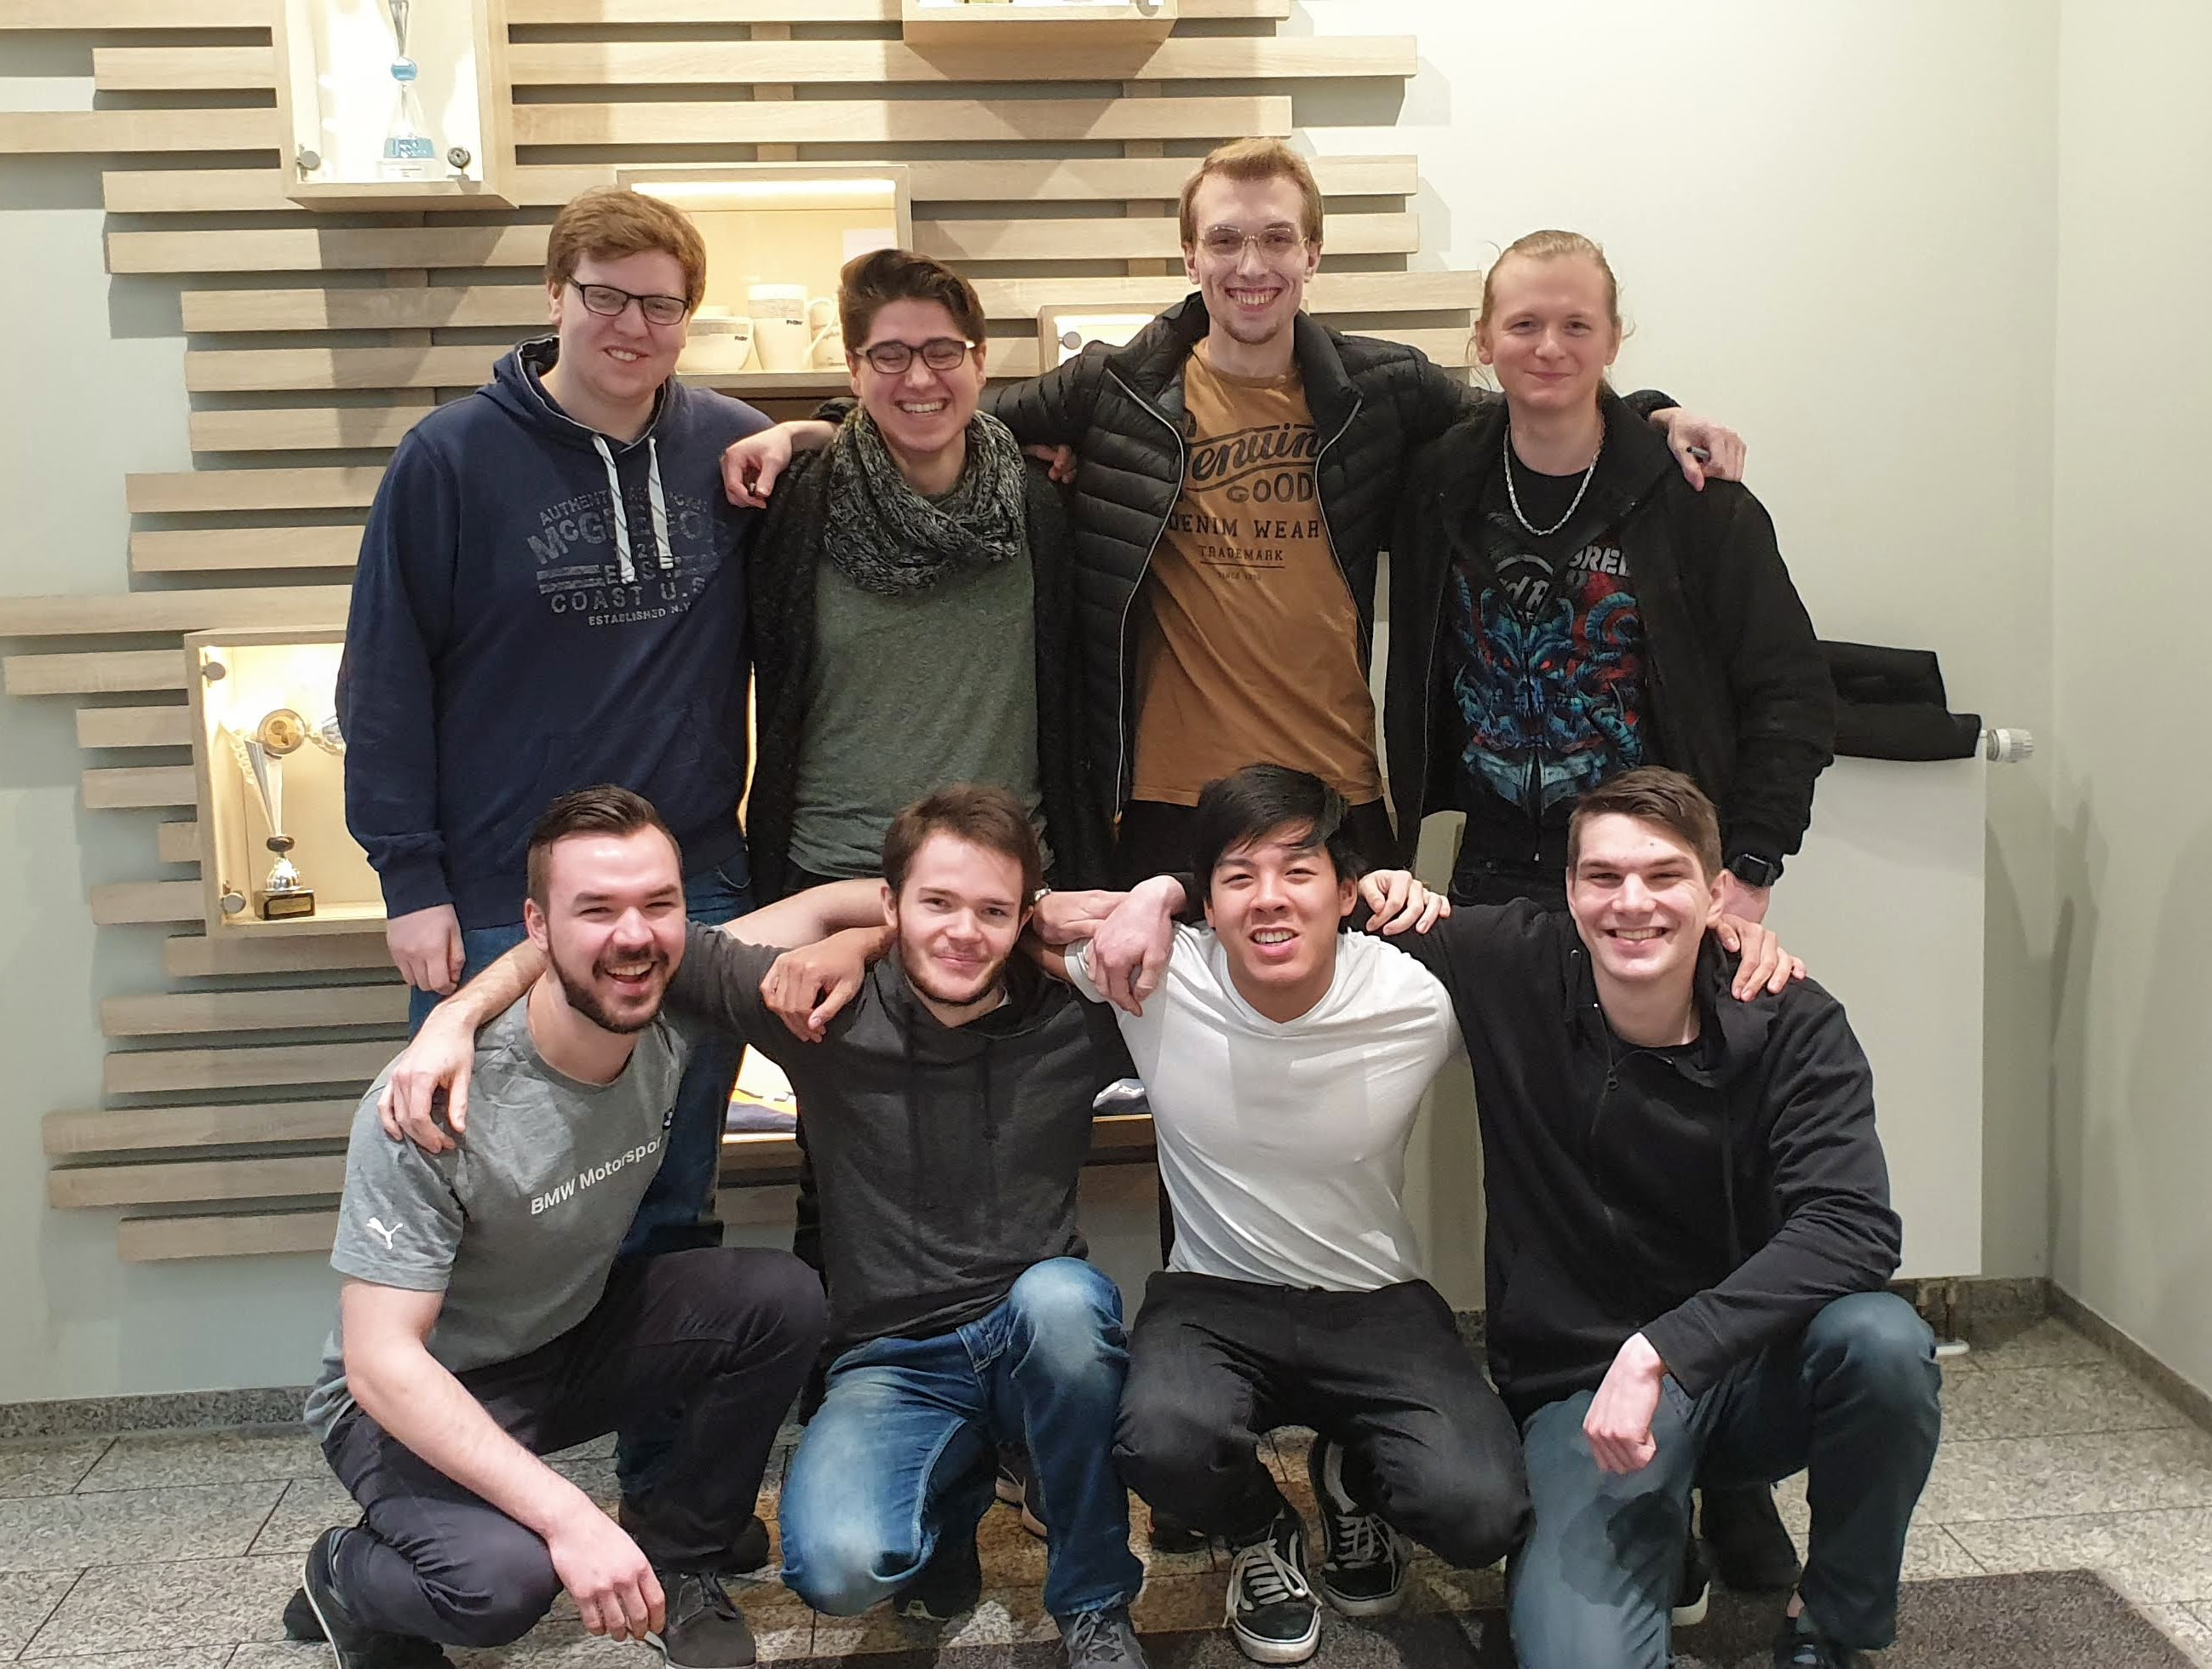
\includegraphics[width=\columnwidth]{img/teamfoto}
	\captionof{figure}{Gruppenfoto}\label{fig:gruppenfoto}
\end{figure}

\vfill

% Adjust this value if we replace images and they suddenly do not fit anymore.
\newcommand{\profilescale}{0.85}

\begin{table}[!htb]
	\centering
	\begin{tabularx}{\columnwidth}{XX}
		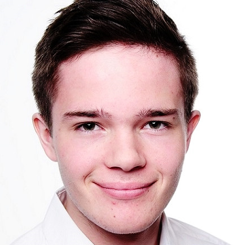
\includegraphics[scale=\profilescale]{img/profil-tom-bockhorn}
		\captionof{figure}{Tom Bockhorn}\label{fig:profil-tom-bockhorn}
			&	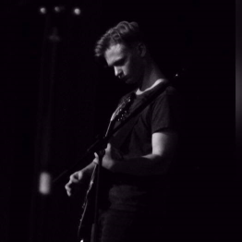
\includegraphics[scale=\profilescale]{img/profil-hendrik-falk}
				\captionof{figure}{Hendrik Falk}\label{fig:profil-hendrik-falk} \\
				
		
\includegraphics[scale=\profilescale]{img/profil-dennis-gentges}
		\captionof{figure}{Dennis Gentges}\label{fig:profil-dennis-gentges}
			&	
\includegraphics[width=8.5em]{img/profil-getuart-istogu}
				\captionof{figure}{Getuart Istogu}\label{fig:profil-getuart-istogu} \\
				% xxx groesse von getis bild anpassen? Warum ist das groesser?
		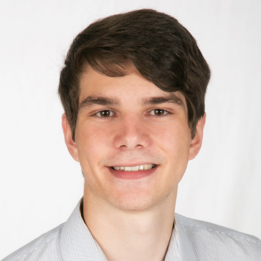
\includegraphics[scale=\profilescale]{img/profil-jannis-keienburg}
		\captionof{figure}{Jannis Keienburg}\label{fig:profil-jannis-keienburg}
			&	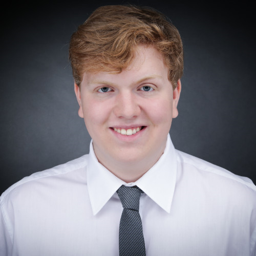
\includegraphics[scale=\profilescale]{img/profil-tim-meinerzhagen}
				\captionof{figure}{Tim Meinerzhagen}\label{fig:profil-tim-meinerzhagen}	\\
				
		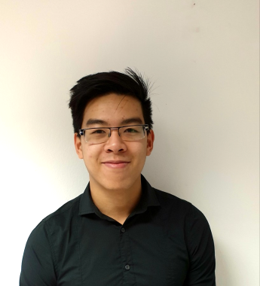
\includegraphics[scale=\profilescale]{img/profil-khang-pham}
		\captionof{figure}{Khang Pham}\label{fig:profil-khang-pham}
			&	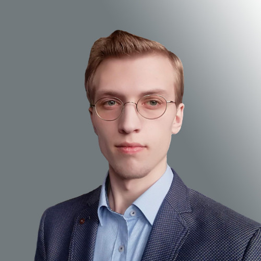
\includegraphics[scale=\profilescale]{img/profil-tim-schwenke}
				\captionof{figure}{Tim Schwenke}\label{fig:profil-tim-schwenke} \\
	\end{tabularx}
\end{table}

